\PassOptionsToPackage{table}{xcolor}
\documentclass[9pt,xcolor=x11names,compress]{beamer}

%% General document %%%%%%%%%%%%%%%%%%%%%%%%%%%%%%%%%%
\usepackage{graphicx}
\usepackage{tikz}
\usepackage{array}
\usetikzlibrary{decorations.fractals,lindenmayersystems,shadings}
%%%%%%%%%%%%%%%%%%%%%%%%%%%%%%%%%%%%%%%%%%%%%%%%%%%%%%


%% Beamer Layout %%%%%%%%%%%%%%%%%%%%%%%%%%%%%%%%%%
\useoutertheme[subsection=false,shadow]{miniframes}
\useinnertheme{default}
\usefonttheme{serif}
\usepackage{palatino}

\setbeamerfont{title like}{shape=\scshape}
\setbeamerfont{frametitle}{shape=\scshape}

\setbeamercolor*{lower separation line head}{bg=DeepSkyBlue4} 
\setbeamercolor*{normal text}{fg=black,bg=white} 
\setbeamercolor*{alerted text}{fg=DeepSkyBlue4} 
\setbeamercolor*{example text}{fg=black} 
\setbeamercolor*{structure}{fg=black} 

\setbeamercolor*{palette tertiary}{fg=black,bg=black!10} 
\setbeamercolor*{palette quaternary}{fg=black,bg=black!10} 

\setbeamertemplate{blocks}[rounded][shadow=true]
\setbeamercolor{block title}{bg=DeepSkyBlue4}
\setbeamercolor{block title example}{bg=DeepSkyBlue4}
\setbeamercolor{block body}{bg=black!15!white}
\setbeamercolor{block body example}{bg=black!15!white}

\setbeamertemplate{navigation symbols}{}
%%%%%%%%%%%%%%%%%%%%%%%%%%%%%%%%%%%%%%%%%%%%%%%%%%
% Some useful definitions
\newcommand*\Laplace[1]{\mathcal{L}\{{#1}\}}
\newcommand*\BLaplace[1]{\mathcal{L}\Big\{{#1}\Big\}}
\newcommand*\iLaplace[1]{\mathcal{L}^{-1}\{{#1}\}}
\newcommand*\ibLaplace[1]{\mathcal{L}^{-1}\big\{{#1}\big\}}
\newcommand*\iBLaplace[1]{\mathcal{L}^{-1}\Big\{{#1}\Big\}}
%%%%%%%%%%%%%%%%%%%%%%%%%%%%%%%%%%%%%%%%%%%%%%%%%%

\author[Francisco Blanco-Silva]{Francisco Blanco-Silva}
\institute[USC]{University of South Carolina}
\date{ 
\pgfdeclarelindenmayersystem{bush}{
	\rule{F -> FF[-F+F][+F-F]}
}
\begin{center}
\begin{tikzpicture}[color=DeepSkyBlue4,rotate=90]
    \draw [l-system={bush, axiom=F, order=5, step=1.6pt, angle=60}]
    lindenmayer system; 
	\end{tikzpicture}	
\end{center}
}

\title{Lesson 22: Systems of differential equations: Numerical methods} 

\begin{document}

\frame{\titlepage}

\section{What do we know?}
\subsection{General Program}

\begin{frame}\frametitle{What do we know?}
\begin{columns}[T]
\begin{column}{0.45\linewidth}
\begin{itemize}
\item The concepts of \alert{differential equation} and \alert{initial value problem}
\item The concept of \alert{order} of a differential equation.
\item The concepts of \alert{general solution}, \alert{particular solution} and \alert{singular solution}.
\item \alert{Slope fields}
\item Approximations to solutions via \alert{Euler's Method} and \alert{Improved Euler's Method}
\end{itemize} 
\end{column}
\begin{column}{0.55\linewidth}
\begin{itemize}
\item First-Order Differential Equations
\begin{itemize}
\item Separable equations 
\item Homogeneous First-Order Equations 
\item Linear First-Order Equations 
\item Bernoulli Equations 
\item General Substitution Methods
\item Exact Equations 
\end{itemize}
\item Second-Order Differential Equations
\begin{itemize}
	\item Reducible Equations
	\item General Linear Equations (Intro)
	\item Linear Equations with Constant Coefficients
	\begin{itemize}
		\item Characteristic Equation
		\item Variation of Parameters
		\item Undetermined Coefficients
	\end{itemize}
\end{itemize}
\end{itemize}
\end{column}
\end{columns}
\end{frame}

\begin{frame}\frametitle{What do we know?}
\framesubtitle{Laplace Transforms}

\noindent\begin{tikzpicture}
\node[scale=0.7]{
\rowcolors{2}{white}{gray!25!white}
	\begin{tabular}{|m{2cm}|m{3.2cm}l||m{2cm}|m{3.2cm}l|}
	\rowcolor{DeepSkyBlue4}
		$f(x)$\raisebox{0.5cm} & $\mathcal{L}\{f\}=\int_0^\infty e^{-sx}f(x)\, dx$\raisebox{0.5cm} & &
		$f(x)$\raisebox{0.5cm} & $\mathcal{L}\{f\}=\int_0^\infty e^{-sx}f(x)\, dx$\raisebox{0.5cm} & \\[0.4cm]
		$1$ & $\dfrac{1}{s}$\raisebox{0.6cm} & $s>0$ &
		$cf(x)\pm g(x)$ & $cF(s) \pm G(s)$\raisebox{0.4cm} & $s>max(a,b)$ \\[0.4cm]
		$x^p$ & $\dfrac{\Gamma(p+1)}{s^{p+1}}$\raisebox{0.6cm} & $s>0$ &
		$x^n f(x)$ & $(-1)^n F^{(n)}$\raisebox{0.4cm} & $s>a$ \\[0.4cm]
		$x^n$ & $\dfrac{n!}{s^{n+1}}$\raisebox{0.6cm} & $s>0$ & $e^{\alpha x}f(x)$ & $F(s-\alpha)$\raisebox{0.4cm} & $s>a+\alpha$ \\[0.4cm]
		$e^{\alpha x}$ & $\dfrac{1}{s-\alpha}$\raisebox{0.6cm} & $s>\alpha$ & $\dfrac{f(x)}{x}$ & $\displaystyle{\int_s^\infty F(\sigma)\, d\sigma}$\raisebox{0.4cm} & $s>a$ \\[0.4cm]
		$\sin \beta x$ & $\dfrac{\beta}{s^2+\beta^2}$\raisebox{0.6cm} & $s>0$  &
		$f\star g$ & $F(s) G(s)$\raisebox{0.4cm} & $s>\max(a,b)$ \\[0.4cm]
		$\cos \beta x$ & $\dfrac{s}{s^2+\beta^2}$\raisebox{0.6cm} & $s>0$ & $f'(x)$ & $s F(s) -f(0)$\raisebox{0.4cm} & $s>a$ \\[0.4cm]
		\hline
		\end{tabular}};
	\end{tikzpicture}
\end{frame}

\begin{frame}\frametitle{What do we know?}
    
\framesubtitle{Systems of Differential Equations}
\begin{equation*}
\underbrace{\begin{cases}
	y_1^{(n)} = F_1\big(x,y_1,y'_1,\dotsc,y_1^{(n-1)}, y_2,y'_2,\dotsc,y_2^{(n-1)},\alert{\dotsb},y_r,y'_r,\dotsc,y_r^{(n-1)}\big) \\
	y_2^{(n)} = F_2\big(x,y_1,y'_1,\dotsc,y_1^{(n-1)}, y_2,y'_2,\dotsc,y_2^{(n-1)},\alert{\dotsb},y_r,y'_r,\dotsc,y_r^{(n-1)}\big) \\
	\dotsc\\
	y_r^{(n)} = F_r\big(x,y_1,y'_1,\dotsc,y_1^{(n-1)}, y_2,y'_2,\dotsc,y_2^{(n-1)},\alert{\dotsb},y_r,y'_r,\dotsc,y_r^{(n-1)}\big)
\end{cases}}_{\text{order }n, r\text{ functions}}
\end{equation*}
\begin{itemize}
	\item Transformation to First-Order systems
	\item Solution by elimination
\end{itemize}
\end{frame}

\section{Warm-up}
\subsection{IVPs}

\begin{frame}\frametitle{Systems of Differential Equations}
\framesubtitle{Initial Value Problems}
\begin{block}
	{Solve the Initial Value Problem. $x=x(t), y=y(t)$}
	\begin{equation*}
	\begin{cases}
		\alert<3>{x'=3x-5y}\\ y'=x-y
	\end{cases}\qquad
	\begin{cases}
		x(0)=1\\y(0)=3
	\end{cases}
	\end{equation*}
\end{block}
\pause We solve the system of differential equations first, by elimination.  The \emph{easier} equation is $y'=x-y$, which gives \alert<4,10>{$x=y'+y$}.  It is then
\begin{equation*}
	y''=\alert<3>{x'}-y'
	\uncover<3->{=\alert<3>{3\alert<4>{x}-5y}-y'}
	\uncover<4->{=3(\alert<4>{y'+y})-5y-y'}
	\uncover<5->{=2y'-2y}
\end{equation*}
\uncover<6->{We need to solve the homogeneous linear equation of second order with constant coefficients $y''-2y'+2y=0$}
\begin{equation*}
	\uncover<7->{r^2-2r+2=0,\qquad r=\frac{2\pm\sqrt{4-4\cdot 2}}{2}=1\pm i}
\end{equation*}
\uncover<8->{It is then $y=e^t\big(A\cos t+B\sin t\big)$}\uncover<9->{, and}
\begin{align*}
	\uncover<10->{x&=y'+y}
	\uncover<11->{=e^t\big(A\cos t + B\sin t\big)+e^t\big( B\cos t-A\sin t\big)+e^t\big(A\cos t + B\sin t\big) \\}
	\uncover<12->{&=e^t\big( (2A+B)\cos t+(2B-A)\sin t \big)}
\end{align*}
\end{frame}

\begin{frame}\frametitle{Systems of Differential Equations}
\framesubtitle{Initial Value Problems}
\begin{block}
	{Solve the Initial Value Problem}
	\begin{equation*}
	\begin{cases}
		x'=3x-5y\\ y'=x-y
	\end{cases}\qquad
	\begin{cases}
		x(0)=1\\y(0)=3
	\end{cases}
	\end{equation*}
\end{block}
\begin{align*}
	x&=e^t\big( (2A+B)\cos t+(2B-A)\sin t \big) \\
	y&=e^t\big( A\cos t + B\sin t \big)
\end{align*}
We need to impose the initial conditions, to find the values of $A$ and $B$ that solve the initial value problem.
\begin{align*}
	1=x(0)&=2A+B\\
	3=y(0)&=A	
\end{align*}
\pause A quick computation gives $A=3, B=-5$, and thus
\begin{align*}
	\alert{x}&\alert{=e^t \big( \cos t-13 \sin t \big)}	 \\
	\alert{y}&\alert{=e^t \big( 3\cos t -5\sin t\big)}
\end{align*}
\end{frame}

\section{Numerical Methods}
\subsection{Euler's Method}

\begin{frame}\frametitle{Systems of Differential Equations}
\framesubtitle{Numerical Methods}
\begin{block}
	{Euler's method for Systems of Differential Equations of First Order}
	Given an initial value problem consisting on a system of $r$ differential equations of first order, with initial conditions
	\begin{equation*}
		\begin{cases}
			y'_1=F_1(x,y_1,y_2,\dotsc,y_r) \\
			y'_2=F_2(x,y_1,y_2,\dotsc,y_r) \\
			\dotsb \\
			y'_r=F_r(x,y_1,y_2,\dotsc,y_r)
		\end{cases}\qquad
	\begin{cases}
		y_1(a_1)=b_1\\ y_2(a_2)=b_2\\ \dotsb \\ y_r(a_r)=b_r
	\end{cases}
	\end{equation*}
	a set number of steps $n$, and a time-step $h>0$, we compute an approximation to the solution $\{y_1,y_2,\dotsc,y_r\}$ with the formula
	\begin{equation*}
		y_j(a_j+hk)=y_j\big( a_j+h(k-1) \big)+h \cdot y'_j\big(a_j+h(k-1)\big) \bigg\rvert_{\substack{j=1,\dotsc,r \\ k=1,\dotsc,n}}
	\end{equation*}
\end{block}
\end{frame}

\begin{frame}\frametitle{Systems of Differential Equations}
\framesubtitle{Numerical Methods}
What we actually compute is a matrix of $r\times n$ values
\begin{center}
\begin{tikzpicture}
\node[scale=0.9]{%
\begin{tabular}{llll}
	$y_{1,1}$ \only<2>{$=b_1$} &
	$y_{2,1}$ \only<2>{$=b_2$} & 
	$\dotsb$  &
	$y_{r,1}$ \only<2>{$=b_r$} \\
	$y_{1,2}$ \only<3>{$=y_{1,1}+h\cdot y'_1(a_1)$} & 
	$y_{2,2}$ \only<3>{$=y_{2,1}+h\cdot y'_2(a_2)$} & 
	$\dotsb$ &
	$y_{r,2}$ \only<3>{$=y_{r,1}+h\cdot y'_r(a_r)$} \\
	$y_{1,3}$ \only<4>{$=y_{1,2}+h\cdot y'_1(a_1+h)$} & 
	$y_{2,3}$ \only<4>{$=y_{2,2}+h\cdot y'_2(a_2+h)$} & 
	$\dotsb$ &
	$y_{r,3}$ \only<4>{$=y_{r,2}+h\cdot y'_r(a_r+h)$} \\
	$y_{1,4}$ \only<5>{$=y_{1,3}+h\cdot y'_1(a_1+2h)$} & 
	$y_{2,4}$ \only<5>{$=y_{2,3}+h\cdot y'_2(a_2+2h)$} & 
	$\dotsb$ &
	$y_{r,4}$ \only<5>{$=y_{r,3}+h\cdot y'_r(a_r+2h)$} \\
	$\dotsb$&
	$\dotsb$&
	$\dotsb$&
	$\dotsb$\\
	$y_{1,n}$ \only<6>{$=y_{1,n-1}+h\cdot y'_1\big(a_1+(n-2)h\big)$} &
	$y_{2,n}$ \only<7>{$=y_{2,n-1}+h\cdot y'_2\big(a_2+(n-2)h\big)$} &
	$\dotsb$ &
	$y_{r,n}$ \only<8>{$=y_{r,n-1}+h\cdot y'_r\big(a_r+(n-2)h\big)$}
\end{tabular}};
\end{tikzpicture}
\end{center}

\vspace{3cm}
\end{frame}

\subsection{Examples}

\begin{frame}\frametitle{Systems of Differential Equations}
\framesubtitle{Numerical Methods}
\begin{block}
	{Use four steps of Euler's method with time-step $h=0.5$ to solve numerically the following IVP:}
	\begin{equation*}
		\begin{cases}
			y'_1=3y_1-5y_2\\
			y'_2=y_1-y_2
		\end{cases}\qquad
		\begin{cases}
			y_1(0)=1\\y_2(0)=3
		\end{cases}
	\end{equation*}
\end{block}
\pause We have $n=4$, $r=2$, $h=0.5$, $(a_1,a_2)=(0,0)$, and $(b_1,b_2)=(1,3)$.  We will use a table to compute all values
\only<2>{\begin{equation*}
	\begin{matrix}
		y_{1,1} & y_{2,1} \\	
		y_{1,2} & y_{2,2} \\	
		y_{1,3} & y_{2,3} \\	
		y_{1,4} & y_{2,4} \\	
	\end{matrix}	
\end{equation*}}
\pause \begin{center}
	\rowcolors{2}{gray!25!white}{white}
	\begin{tabular}{|l|l||c|c||c|c|}
		\rowcolor{DeepSkyBlue4}
		$n$ & $x$ & $y_1$ & $y_2$ & $y'_1$ & $y'_2$ \\
		$1$ & $0$ & \alert{$1$} & \alert{$3$} & \only<4>{$3\cdot 1-5\cdot 3$}\only<5->{$-12$} & \only<4>{$1-3$}\only<5->{$-2$} \\
		$2$ & \only<5->{$0.5$} & \only<6>{$1+0.5\cdot (-12)$}\only<7->{\alert{$-5$}} & \only<6>{$3+0.5\cdot (-2)$}\only<7->{\alert{$2$}} & \only<8>{$3\cdot (-5)-5\cdot(2)$}\only<9->{$-25$} & \only<8>{$-5-2$}\only<9->{$-7$}\\
		$3$ & \only<9->{$1$} & \only<10>{$-5+0.5\cdot (-25)$}\only<11->{\alert{$-17.5$}} & \only<10>{$2+0.5\cdot(-7)$}\only<11->{\alert{$-1.5$}} & \only<12>{$3\cdot (-17.5)-5 \cdot (-1.5)$}\only<13->{$-45$}& \only<12>{$-17.5+1.5$}\only<13->{$-16$} \\
		$4$ & \only<13->{$1.5$} & \only<14>{$-17.5+0.5\cdot(-45)$}\only<15->{\alert{$-40$}}& \only<14>{$-1.5+0.5\cdot(-16)$}\only<15->{\alert{$-9.5$}}& &  \\
		\hline
	\end{tabular}
\end{center}
\end{frame}

\begin{frame}\frametitle{Systems of Differential Equations}
\framesubtitle{Numerical Methods}
\begin{block}
	{Use four steps of Euler's method with time-step $h=0.5$ to solve numerically the following IVP:}
	\begin{equation*}
		\begin{cases}
			y'_1=3y_1-5y_2\\
			y'_2=y_1-y_2
		\end{cases}\qquad
		\begin{cases}
			y_1(0)=1\\y_2(0)=3
		\end{cases}
	\end{equation*}
\end{block}
\begin{center}
\begin{tabular}{c}
	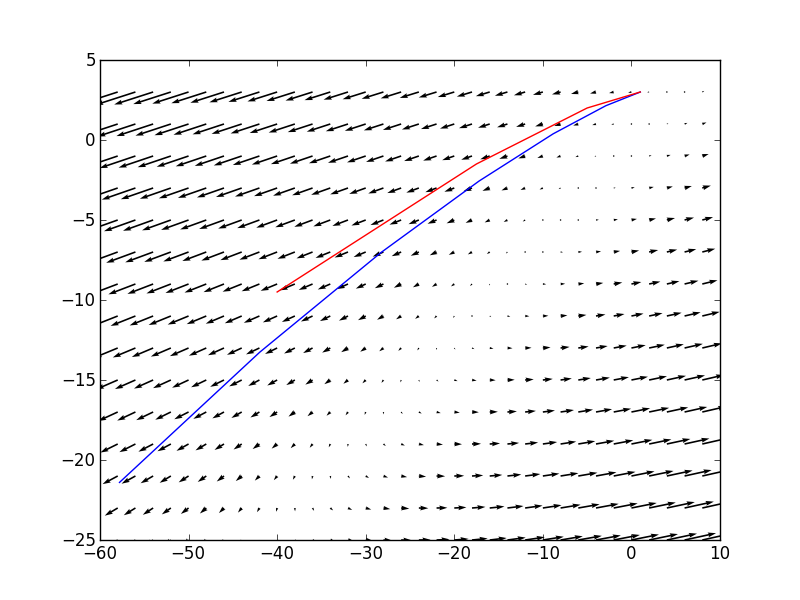
\includegraphics[height=0.4\linewidth]{lesson22ma242.png} \\
	\tikz\draw[blue,thick](0,0)--(0.5,0);
	Actual solution $\boldsymbol{y}(x)=\big( y_1(x),y_2(x)\big)$ \hspace{0.5cm}\, \\
	\tikz\draw[red,thick] (0,0)--(0.5,0);
	Numerical Solution with Euler's Method
\end{tabular}
\end{center}
\end{frame}
\end{document}
 347.76